\section{Об оффлайн деревьях поиска: введение}

Исходная статья: ``The Geometry of Binary Search Trees''~\cite{demaine2009geometry}.

\subsection{Оффлайн деревья поиска и графическое представление}

Пусть у нас есть дерево над ключами $1$, $2$, \ldots, $n$ и последовательность $S = (s_1, s_2, \ldots, s_m)$ запросов поиска. Запросы нам известны заранее и мы хотим построить такое дерево, чтобы минимизировать суммарное время, потраченное на то, чтобы ответить на эти запросы. 
%Обычно считается, что $m \geqslant n$ и, более того, мы потрогали каждый ключ хотя бы один раз, но я этого дальше делать не буду. 
При этом мы разрешаем перестраивать дерево с помощью вращений в процессе 
ответа на запросы.

Нам разрешено делать следующие вещи:
\begin{enumerate}
\item Переходить по указателю.
\item Делать одинарное вращение с центром в этой вершине (zig, он же zag).
\end{enumerate}

Начинаем при этом мы всегда в корне, а для каждого запроса хотим посетить вершину
с соответствующим ключом.

\newdefn{Последовательность таких действий для фиксированной последовательности 
запросов $S$ называется \emph{BST-алгоритмом}.}

\newdefn{Цена операции поиска~--- количество посещённых узлов. Поскольку для того, чтобы сделать вращение в вершине, нам нужно её посетить, учитывать количество вращений не нужно, если мы считаем с точностью до константы.}

\newdefn{$\opt(S)$~--- минимальная суммарная цена выполнения $S$, если мы заранее знаем $S$ и можем в связи с этим выбирать, какие именно операции вращения
мы будем делать, а какие~--- нет (а также можем выбрать, как дерево выгляд} 

Значение 
$\opt(S)$ мы не умеем искать (даже с точностью до мультипликативной
константы) за полином. Впрочем, опровергать возможность вычисления $\opt(S)$ 
за полином мы тоже не умеем, даже в предположении $\P \neq \NP$. Ясно,
что задача о проверке неравенства $\opt(S) \leqslant k$ лежит в $\NP$.

Это можно переформулировать в геометрических терминах. Рассмотрим координатную
плоскость с ключами по оси $x$ и моментами времени (то есть номерами запросов) по 
оси $y$. Для данной последовательность запросов $S$ отметим все точки $(s_i, i)$ 
на плоскости (мы обязаны посетить ключ $s_i$ при обработке $i$-того
запроса, так как мы должны его найти). Также отметим все точки $(k, i)$ такие,
что мы посетили ключ $k$ при обработке $i$-того запроса. Понятно, что стоимость данной
последовательность операций~--- количество отмеченных точек.

\newdefn{Множество отмеченных точек~--- \emph{графическое представление} данного BST-алгоритма. У разных BST-алгоритмов могут быть одинаковые представления.}	

% Е, ужасная подгонка констант!

\begin{figure}
    \centering
    \begin{tabular}{cc}
    
    \begin{subfigure}{0.6\textwidth} 
        \centering
        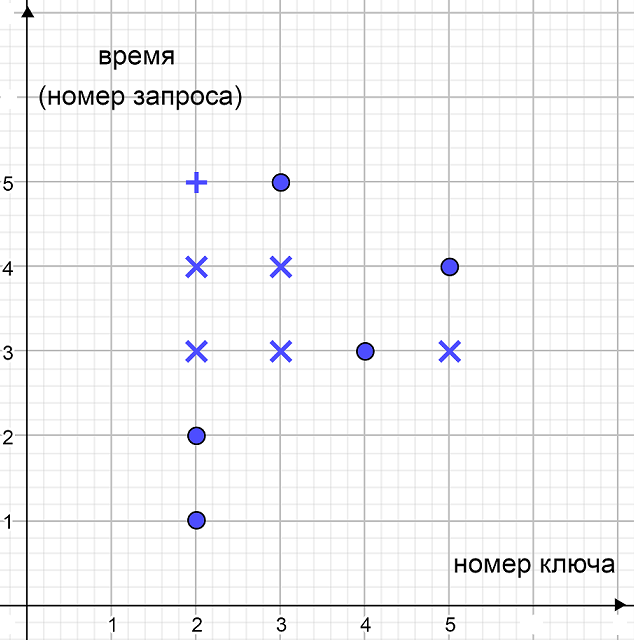
\includegraphics[height=5cm]{img/graph_repr_example.png}
        \caption{Графическое представление BST-алгоритма: жирными точками отмечены сами запросы, крестиками и плюсиком~--- другие ключи, которые мы посещаем в процессе их обработки. От плюсика можно избавиться, см. основной текст.}
        \label{repr_example_graph}
    \end{subfigure}
    
    &
    
    \begin{subfigure}{0.4\textwidth} 
        \centering
        \begin{subfigure}{0.4\textwidth}
        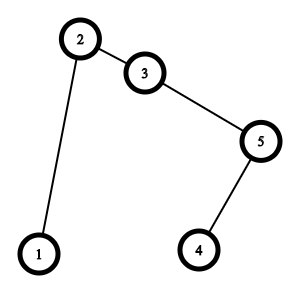
\includegraphics[height=3cm]{img/tree_original.png}
        \caption{Исходное дерево.}
        \label{repr_example_orig}
        \end{subfigure}
        
        \begin{subfigure}{0.4\textwidth}
        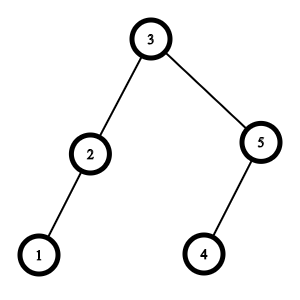
\includegraphics[height=3cm]{img/tree_rebuild.png} 
        \caption{Дерево после операции \textrm{rotate 3}.}
        \label{repr_example_rebuild}
        \end{subfigure}
    \end{subfigure}
    
    \\
    \end{tabular}
    \caption{Пример графического представления}
    \label{repr_example}
\end{figure}

На рисунку~\ref{repr_example_graph} видно графическое представление, которое получится, 
если для дерева с рисунка~\ref{repr_example_orig}
применить последовательность запросов $S = (2, 2, 4, 5, 3)$ и при этом не совершать
никаких вращений. От плюсика можно избавиться, если 
при обработке четвёртого запроса сделать операцию \textrm{rotate 3} и получить дерево с рисунка~\ref{repr_example_rebuild} (в таком дереве для обработки запроса \textrm{найти ключ 3} не нужно посещать вершину с ключом $2$, так как вершина с ключом $3$ уже является корнем).

Про splay-деревья верят, что они оптимальны с точностью до мультипликативной константы,
то есть что они посещают $O(\opt(S) + n)$ вершин при обработке любого списка запросов $S$.
Это достаточно круто, так как splay-деревья не знают будущего,
в отличие от оптимальное алгоритма. Однако, доказывать это про splay-деревья не умеют,
но есть другие деревья, про которые это умеют доказывать.

\newdefn{Если $a$ и $b$~--- точки на плоскости, то $\rect(a, b)$~--- прямоугольник (возможно, вырожденный), натянутый на точки $a$ и $b$ как на противоположные углы.}

\newdefn{Множество целых точек на плоскости $E$ называется \arbs,
если для любых точек $a$ и $b$ из $E$ верно хотя бы одно из следующих трёх свойств: $x(a) = x(b)$, $y(a) = y(b)$ или $\rect(a, b)$ содержит точку из $E \setminus \set{a, b}$.}

\subsection{Эквивалентность BST-алгоритмов и \arbs множеств}

\begin{theorem}\label{bst_to_arbs} Если множество точек $E$ может быть отмечено каким-то BST-алгоритмом,
то оно \arbs.
\end{theorem}
\begin{proof} Предположим противное. Пусть мы нашли две точки $a$ и $b$, при этом
$x(a) \neq x(b)$, $y(a) \neq y(b)$ и внутри $\mathrm{rect}(a, b)$ нет других точек $E$. 
Не умаляя общности, $i \coloneqq y(a) < y(b)\eqqcolon j$. Пусть $c$~--- наименьший общий предок $a$ и $b$ \emph{после} обработки $i$-того запроса.
Есть два случая:
\begin{enumerate}
\item Если $c = a$, то мы должны были посетить $a$ в какой-то момент из отрезка $(i + 1, j]$. Действительно, раз $a$ является предком $b$ после обработки $i$-того запроса, то либо $a$~--- всё ещё предок $b$ \emph{перед} обработкой $j$-того запроса (и тогда мы должны посетить $a$ просто для того, чтобы дойти до $b$), либо вершина $a$ перестала быть предком $b$ в какой-то из моментов на отрезке $(i + 1, j)$, а для этого мы должны были её посетить и сделать вращение в её ребёнке.

\item Если $c \neq a$, то $a$ и $b$ лежат в разных поддеревьях $c$. Следовательно, по свойству двоичного дерева поиска, $x(c) \in \langle x(a), x(b) \rangle$ (ключ вершины $c$ должен лежать между ключами вершин $a$ и $b$; здесь $\langle s, t \rangle$ это либо $[s, t]$, если $s < t$, либо $[t, s]$ в противном случае). Раз мы посетили $a$ при обработке $i$-того
запроса, то мы посетили и её предка $c$, следовательно множество $E$ содержит точку $(x(c), y(c)) = (x(c), i)$, а она лежит в искомом прямоугольнике.
\end{enumerate}
\end{proof}

Стоит заметить, что мы доказали более сильный факт: если $x(a) \neq x(b)$ и $y(a) \neq y(b)$, то есть точка из $E \setminus \{a \}$, которая попала на одну из сторону $\rect(a, b)$, смежную с $a$ (то, какая это сторона, зависит от того, $c = a$ или $c \neq a$). Аналогичное утверждение верно для $E \setminus \{ b \}$ и $b$. 

Дальше мы будем постоянно пользоваться следующей леммой, утверждающей, что описанное в прошлом абзаце условие верно для любого \arbs множества, а не только для тех, которые
являются графическим представлением BST-алгоритма (позже мы поймём, что каждое
\arbs множество~--- графическое представление какого-то BST-алгоритма, но не будем торопить события).

\begin{lemma}\label{strong_arbs} Если $E$~--- \arbs, то для любых $a$ и $b$ из $E$, таких что $x(a) \neq x(b)$ и $y(a) \neq y(b)$, существует точка из $E \setminus \{a \}$, которая попадает на одну из сторон 
$\rect(a, b)$ 
\end{lemma}
\begin{proof} Пусть у нас есть $\rect(a, b)$ для точек $a$ и $b$, удовлетворяющих 
условиям $x(a) \neq x(b)$ и $y(a) \neq y(b)$. Так как $E$~--- \arbs множество, то есть
$c \in \rect(a, b)$, $c \neq a$ и $c \neq b$. Есть два случая:
\begin{enumerate}
\item $x(c) = x(a)$ или $y(c) = y(a)$. Тогда $c$ лежит на одной стороне $\rect(a, b)$
с точкой $a$, то есть $c$~--- искомая точка.
\item $x(c) \neq x(a)$ и $y(c) \neq y(a)$. Тогда в $\rect(a, c)$ тоже есть точка из $E \setminus \{a, c \}$ по обычному \arbs свойству, при этом $\rect(a, c)$ строго меньше
$\rect(a, b)$. Будем повторять процесс (возьмём точку $d \neq a$, $d \neq c$ из $\rect(a, c)$,
и так далее), пока неизбежно не выполнится случай $1$.
\end{enumerate}
\end{proof}

Немного удивительно, но верна и теорема, обратная к теореме~\ref{bst_to_arbs}:
теорема~\ref{arbs_to_bst}. Для её доказательства нам понадобится понимать
некоторые базовые вещи про декартовы деревья.

\newdefn{\emph{Декартово дерево}~--- это двоичное дерево поиска, в котором у каждой
вершины кроме ключа есть ещё и другой параметр~--- \emph{приоритет}, при этом
декартово дерево образуют кучу на минимум по приоритетам.}

\newdefn{Декартово дерево на парах $(\mathrm{key}_i, \mathrm{priority}_i)$~--- любое декартово дерево с данными мультимножеством пар  ``ключ--приоритет''.}	

\begin{lemma} Всегда есть хотя бы одно декартово дерево на данном наборе пар.
Более того, если все ключи и приоритеты в наборе различны, то
декартово дерево только одно.
\end{lemma}
\begin{proof} По свойству кучи корнем декартова дерева должна быть одна из вершин с минимальным приоритетом. Возьмём любую вершину с минимальным приоритетом и сделаем её корнем, пусть её \emph{ключ} равен $x$. Тогда все вершины с ключами меньше $x$ должны попасть в её левое поддерево, а с ключами больше $x$~--- в правое. Куда попадут вершины с ключом ровно $x$, неважно. Распределим оставшиеся вершины на левое и правое поддерево корня и построим их рекурсивно. Если все ключи и приоритеты были различны, то каждый раз мы делали единственное возможное действие, поэтому в этом случае декартово дерево уникально.
\end{proof}

Также нам понадобится следующая лемма.

\begin{lemma}\label{tree_distance} Пусть у нас есть два двоичных дерева поиска на одном и том же наборе из $n$ ключей. Тогда одно из них можно перестроить в другое, сделав $O(n)$ вращений.
\end{lemma}
\begin{proof} Самое интуитивное доказательство этого факта использует соответствие
между двоичными деревьями поиска на $n$ вершинах и триангуляциями $(n + 2)$-угольника.

Соответствие выглядит так: зафиксируем любую сторону многоугольника и назовём её \emph{корневой стороной}. Оставшиеся $n$ вершин, не попавшие на корневую сторону,
пронумеруем по циклу числами от $1$ до $n$. Пусть теперь у нас есть 

\todo{дописать}
\end{proof}

\begin{theorem}\label{arbs_to_bst} Если $E$~--- \arbs, то существует BST-алгоритм, графическое представление
которого в точности равно $E$. Строго говоря, нужно ещё не забыть наложить
условие, что множество $y$-координат точек из $E$~--- в точности отрезок целых чисел $[1, n]$ для какого-то $n$. Это соответствует тому, что при каждом запросе мы должны обязательно посетить корень, то есть хотя бы одну вершину.
\end{theorem}
\begin{proof} Обозначим за $\tau_i$ множество из ключей, которые нам разрешено посещать на $i$-том шаге (то есть такие ключи $x$, что $(x, i) \in E$).

В момент времени $i$ наше дерево будет \emph{каким-то} (не любым, а именно каким-то; то есть ``существует последовательность декартовых деревьев'', а не ``для любой последовательности декартовых деревьев'') декартовым деревом на парах $(x, N(x, i))$, где $N(x, i)$~--- минимальное такое $j \geqslant i$, что $(x, j) \in E$ или $+\infty$, если таких $j$ нет. Интуитивно, $N(x, i)$ должно быть первым моментом времени, начиная с $i$, когда мы посетим ключ $x$. $T_1$~--- какое-то декартово дерево, хотим перестроить $T_i$ в $T_{i+1}$, посетив только вершины из $\tau_i$.

Вершины, которые мы можем посещать в момент времени $i$~--- какой-то связный кусок $T_i$, содержащий корень $T_i$. Почему? Потому что у всех вершин $T_i$ приоритет равен $N(x, i)$, то есть хотя бы $i$, а у вершин из $\tau_i$ приоритет равен ровно $i$. При этом только
у вершин из $\tau_i$ приоритет поменяется на что-то новое (так как для других ключей $N(x, i) = N(x, i + 1)$).  Назовём вершины из $\tau_i$ \emph{верхними}, а все остальные~--- \emph{нижними}.

Дерево $T_i$ устроено следующим образом: это какое-то дерево поиска (назовём его \emph{верхней компонентой}) на вершинах из $\tau_i$, только вместо некоторых ``пустых детей'' (то есть вместо \textrm{nullptr}'ов) подклеены \emph{нижние поддеревья}~--- поддеревья, целиком состоящие из нижних вершин. Чтобы получить $T_{i+1}$ из $T_i$, перестроим верхнюю компоненту в соответствии с новыми приоритетами вершин из $\tau_i$ (это можно сделать по лемме~\ref{tree_distance}) с помощью вращений. Строго говоря, лемма даёт нам последовательность вращений верхней компоненты, но каждое вращение верхней компоненты естественным образом является вращением и всего дерева тоже. Поскольку мы использовали только вращения, свойство двоичного дерева поиска не начало нарушаться.

Теоретически, могло нарушится условие кучи. Поскольку все верхние вершины остались наверху, а нижние~--- внизу, то в $T_{i+1}$ может быть лишь три типа пар ``родитель-сын'', где нарушилось условие кучи: ``верх-верх'', ``низ-низ'' и ``верх-низ''. Нарушений типа ``верх-верх''
нет, поскольку $T_{i+1}$ строилось так, чтобы для верхних вершин в нём выполнялось условие кучи с новыми приоритетами. Нарушений типа ``низ-низ'' нет, так как при вращениях вершин из $\tau_i$ нижние поддеревья могли как-то переставляться, но при этом их внутренняя структура не менялась, так как мы не трогали нижние вершины. Осталось понять, почему не могло быть нарушений вида ``верх-низ''. Тут-то нам и пригодится то, что $E$~--- \arbs.

Пусть в $T_{i+1}$ есть нижняя вершина с парой ``ключ--приоритет'' $(y, j)$ и её родитель~--- верхняя вершина с парой $(x, k)$. Раз эти вершины нарушают свойство кучи, то $j < k$.
Не умаляя общности, $x < y$. Посмотрим на точки $(x, i)$ и $(y, j)$ из $E$ и натянутый на них прямоугольник $\rect((x, i), (y, j))$. На вертикальной стороне от $(x, i)$ до $(x, j)$ нет ничего из $E \setminus \{(x, i) \}$ по определению, так как $N(x, i + 1) = k > j$. Следовательно, по лемме~\ref{strong_arbs}, есть точка $(c, i)$ на
стороне от $(x, i)$ до $(y, i)$. Это значит, что $c \in \tau_i$, то есть $c$~--- верхняя вершина.

Все наши операции при перестройке $T_i$ в $T_{i+1}$ были вращениями: они могли сломать свойство кучи, но не свойство двоичного дерева поиска. Поэтому, ключ $c$ всё ещё лежит между ключами $x$ и $y$. Но вершина с ключом $y$~--- родитель вершины с ключом $x$ в $T_{i+1}$. Следовательно, вершина с ключом $c$ находится где-то в правом поддереве вершины $y$ дерева $T_{i + 1}$. Это невозможно, так как $c$~--- верхняя вершина и должна была остаться наверху (но не осталась, так как она отделена нижней вершиной $y$ от верхней вершины $x$). Противоречие.
\end{proof}

\subsection{``Онлайн-эквивалентность'' BST-алгоритмов и \arbs множеств}

Только что мы получили оффлайн-алгоритм, который, зная \arbs множество $E$, строит BST-алгоритм с графическим представлением $E$. Утверждается, что есть \emph{онлайн}-алгоритм который, получая не всё $E$ сразу, а по строкам (получил $\tau_1$, сделал нужные операции, получил $\tau_2$, сделал нужные операции, и так далее)), строит BST-алгоритм со стоимостью $O(|E| + n)$ 	
(получить в точности графическое представление $E$ не получится, ухудшения на мультипликативную константу не избежать). Здесь, как и в прошлом разделе, под $\tau_i$
понимается множество таких ключей $x$, что $(x, i) \in E$.

Нам понадобится немного необычная структура данных.

\newdefn{
\emph{split-дерево} (\textrm{split-tree})~--- это абстрактная структура данных, состоящая из \emph{внутреннего двоичного дерева поиска} на имеющихся ключах и какой-то \emph{дополнительной информации}, которая может иметь любую природу. При этом она должна уметь поддерживать две операции:
\begin{enumerate}
\item \textrm{make\_tree}($x_1$, $x_2$, \ldots, $x_n$)~--- по отсортированному массиву ключей построить структуру данных, при этом внутреннее дерево поиска должно быть двоичным деревом поиска на данных ключах;
\item \textrm{split\_tree}($x$)~--- найти ключ $x$ во внутреннем двоичном дереве поиска (гарантируется, что он там есть), с помощью вращений поднять его в корень, удалить его и вернуть два новых split-дерева: левое и правое поддеревья корня (в левом все ключи меньше $x$, а в правом все ключи больше $x$).
\end{enumerate}
При этом разрешается тратить суммарно только $O(n)$ времени на построение (\textrm{make\_tree})
и полное разрушение ($n$ операций \textrm{split\_tree}) дерева.
}

\begin{remark}[Небольшое отступление о природе split-дерева.] Операции ``постройте структуру по списку чисел'' и ``найдите данное число в структуре, удалите его и разбейтесь на <<до>> и <<после>>'' можно легко реализовать с помощью односвязного списка и хэш-таблицы или кучи других подобных методов.

Но суть split-дерева не в этом. Суть split-дерева в том, что оно реализует операцию \textrm{split\_tree} \emph{физически} на внутреннем двоичном дереве поиска с помощью вращений в точности так, как описано. Вся дополнительная информация, которую мы храним, существует не для того, чтобы отвечать на какие-то запросы об элементах структуры, а только для того, чтобы лучше понимать, как и когда совершать дополнительные вращения, кроме тех, которые нам нужны, чтобы пригнать ключ $x$ в корень.

Нас интересует не столько время, которые мы потратили, сколько число вершин во внутреннем двоичном дереве, которые мы затронули. Если бы мы могли потратить $O(n^2)$ времени, но затронуть вершины только $O(n)$ раз в процессе полного разрушения внутреннего дерева, это бы нас более-менее устроило. Но оказывается, что мы можем потратить $O(n)$ времени (и, следовательно, лишь $O(n)$ раз затронуть вершины внутреннего дерева). Раз можем, то почему бы и не воспользоваться чуть лучшей версией алгоритма?

Я не буду воспроизводить принцип работы split-дерева, так как он не очень важен. Узнать его можно в исходной статье~\cite{demaine2009geometry}. Более того, есть гипотеза (см. статью Лукас~\cite{lucas1988canonical}), что в качестве split-дерева можно использовать обыкновенное splay-дерево без дополнительной информации (и, соответственно, не делать никаких вращений, кроме тех, которые нужны, чтобы пригнать ключ в корень), но доказывать это не умеют.
\end{remark}

Теперь мы будем на каждом шаге строить не обычное декартово дерево, а обобщённое декартово дерево (определение в следующем абзаце). $G_i$~---
обобщённое декартово дерево (с отличием, что теперь мы просим, чтобы декартово дерево было кучей на \emph{максимум} по приоритетам), построенное на парах $(x, \rho(x, i))$, где $\rho(x, i)$~--- максимальное такое $j < i$, что $(x, j) \in E$ или $-\infty$, если таких нет. То есть $\rho(x, i)$~--- последний момент строго перед $i$, когда ключ $x$ был задет. Фактически, мы повернули вспять течение времени и сделали так, что теперь вершины с большими $\rho(x, i)$ находятся выше в дереве (раньше~--- вершины с меньшими $N(x, i)$). Однако, не всё так просто, так как теперь вершины, у которых мы меняем приоритет расположены внутри дерева, на первый взгляд, как-то случайно.

\newdefn{\emph{Обобщённое декартово дерево} (\textrm{general treap})~--- это на самом деле обычное декартово дерево, вершины которого объединены в \emph{суперузлы}:
\begin{enumerate}
\item Каждый суперузел~--- связное подмножество вершин дерева с одинаковым приоритетом.
Для одного приоритета может быть несколько суперузлов, но они должны быть не связаны между собой (то есть соседние вершины с одинаковым приоритетом обязаны попасть в один и тот же суперузел).
\item Каждый суперузел~--- split-дерево (точнее, внутреннее двоичное дерево для split-дерева). Гарантируется, что суперузлы создаются с помощью операции \textrm{make\_tree}, а потом постепенно разрушаются с помощью операций \textrm{split\_tree}. Так как внутри суперузла все приоритеты одинаковые, то любое двоичное дерево поиска будет удовлетворять условию кучи. 
\end{enumerate}
}

\newdefn{Отношение ``отец--сын'' на суперузлах определяется естественным образом. При этом у суперузла (в отличие от обычной вершины) может быть много детей.}

\begin{remark} Важно понимать, что суперузлов в некотором смысле ``не существует''~--- обобщённое декартово дерево не является двумерной структурой данных в любом привычном смысле слова. Как уже было сказано, обобщённое декартово дерево по своей внутренней структуре~--- обычное декартово дерево.
Суперузлы мы выделили сами, чтобы внутри них строить split-деревья и пользоваться амортизированной оценкой из определения split-деревьев.

На это можно смотреть так: все наши ключи различны, но среди приоритетов есть одинаковые, и их достаточно много. Поэтому в структуре декартова дерева есть некоторая свобода, связанная с тем, как именно мы располагаем соседние вершины с одинаковым приоритетом. Мы воспользовались этой свободой, чтобы построить в каждом суперузле split-дерево, которое будет нам говорить, как именно расположены вершины этого суперузла.
\end{remark}

Изначально, $G_1$ состоит из одного суперузла с приоритетом $-\infty$, который мы строим с помощью \textrm{make\_tree}. 
Как получить $G_{i+1}$ из $G_i$? Для этого нужно взять все
вершины из $\tau_i$, так как только для них $\rho(x, i+1) \neq \rho(x,i)$ (а именно, $\rho(x, i + 1) = i$ для $x \in \tau_i$; для других вершин $\rho(x, i + 1) = \rho(x, i) < i$), 
вырезать их из своих суперузлов с помощью \textrm{split\_tree} и собрать из них новый суперузел с приоритетом $i$ с помощью \textrm{make\_tree}. Строгое понимание этих слов (в частности, то, как мы поддерживаем при всех этих операциях свойства обобщённого декартово дерева и даже то, почему $G_{i+1}$ вообще окажется хотя бы обычным декартовым деревом) отложим на потом. А пока сделаем ещё одно полезное замечание о split-деревьях.

\begin{remark} 
Split-дерево в процессе своей работы производит какие-то операции вращения внутреннего двоичного дерева поиска. Но эти операции вращения (выполнить вращения в какой-то вершине) можно совершать и со связными подмножествами большего дерева поиска, в нашем случае обобщённого декартова дерева.

То есть внутренние деревья поиска наших split-деревьев~--- какие-то куски нашего
обобщённого декартового дерева, а именно, суперузлы. В частности, эти внутренние
деревья не нужно хранить отдельно, так как они сохранены в нашем декартовом дереве.
Когда split-дерево говорит, что нам нужно сделать вращение во внутреннем дереве, мы делаем вращение в соответствующей вершине нашего большого дерева.

При таком понимании у удаления вершины (операции \textrm{split\_tree}($x$)) появляется
следующая интерпретация: мы не столько \emph{удаляем} вершину с ключом $x$, сколько пригоняем её в корень куска большого дерева, соответствующего нашему split-дерева, прекращаем ассоциировать её с нашим split-деревом и чисто формально (дополнительную информацию, если она есть, нужно будет пересчитать, но менять в структуре большого дерева ничего не надо) разбиваем наше split-дерево на два. 

После такой операции наша вершина перестаёт быть ассоциированой с \emph{каким-либо} split-деревом, поэтому мы больше не будем делать вращений с центром в ней до того, как перейдём к $(i+1)$-ой итерации процесса (построению $G_{i+2}$ по $G_{i+1})$. 

Однако, как мы поймём позже, это не помешает ей дойти до корня
\end{remark}

Нам понадобится следующая лемма:

\begin{lemma}\label{visited_parent}
Пусть мы посетили (то есть $x \in \tau_i$) вершину с парой ``ключ--приоритет'' $(x, k)$ в $G_i$. Пусть отец её суперузла (в $G_i$, всё пока в $G_i$)~--- суперузел $P$ с приоритетом $j > k$. 
Пусть $\mathrm{succ}(P, x)$~--- наименьший ключ в $P$, больший $x$, $\mathrm{pred}(P, x)$~--- наибольший ключ в $P$, меньший $x$.
Утверждается, что мы их посетили (если они существуют), то есть $\mathrm{succ}(P, x) = +\infty$ или $\mathrm{succ}(P, x) \in \tau_i$, и, аналогично, $\mathrm{pred}(P, x) \in \tau_i \cup \{-\infty\}$.
\end{lemma}
\begin{proof}
Действительно, пусть $\mathrm{succ}(P, x) < +\infty$ и $\mathrm{succ}(P, x) \notin \tau_i$, откуда $(\mathrm{succ}(P, x), j + 1), (\mathrm{succ}(P, x), j + 2), \ldots, (\mathrm{succ}(P, x), i) \notin E$. Тогда, так как $(x, i) \in E$ и $(\mathrm{succ}(P, x), j) \in E$, то в $E \setminus \{\mathrm{succ}(P, x)\}$ есть точка на стороне $(\mathrm{succ}(P, x), j)$--$(x,j)$ прямоугольника $\rect((x, i), \mathrm{succ}(P, x))$. Следовательно, есть такое $y \in [x, \mathrm{succ}(P, x))$, что $(y, j) \in E$. Так как $\rho(x, i) = k < j$, то $(x, j) \notin E$, откуда $y$ лежит строго между
$x$ и $\mathrm{succ}(P, x)$. 

\begin{figure}
\includegraphics[height=4cm]{img/lemma_proof_diagram.png}

\caption{Зелёные точки соответствуют точкам из $E$, красные отрезки~--- отрезкам, на которых точно нет точек из $E$ из-за того, что мы знаем значения 
$\rho(\cdot, \cdot)$. Точка $(y, j)$ появляется из леммы~\ref{strong_arbs} для $(x, i)$ и 
$(\mathrm{succ}(P, x), j)$.}
\end{figure}

Получается, что $\rho(y, i) \geqslant j$. Почему это странно? Мы уже знаем, что ключ $y$ каким-то образом лежит между ключом $\mathrm{succ}(P, x)$ и ключом $x$. Это означает, что он лежит в поддереве наименьшего общего предка 
$\mathrm{succ}(P, x)$ и $y$. Этот наименьший общий предок~--- какая-то вершина из $P$ (потому что $\mathrm{succ}(P, x)$ лежит в $P$ по определению, а $P$~--- отец суперузла, в котором лежит $x$), следовательно его приоритет \emph{не больше} приоритета $P$, то есть $j$. С другой стороны, мы уже доказали, что $\rho(y, i) \geqslant j$. Отсюда, приоритет $y$ в точности равен $j$ и $y$ лежит в $P$. Но это противоречит определению $\mathrm{succ}(P, x)$, так как $x < y < \mathrm{succ}(P, x)$. Аналогично с $\mathrm{pred}(P, x)$.

%Картинка 2
\end{proof}

Что мы получили? Как минимум то, что множество посещённых \emph{суперузлов} (то есть таких суперузлов, в которых есть вершина из $\tau_i$), образуют связное множество, содержащее корень. Аналогичное утверждение про \emph{вершины} неверно, но оно нам и не понадобится. Сейчас нам понадобится понять ещё одну интересную особенность split-дерева.

Наша цель состоит в том, чтобы небольшим количеством вращений пригнать все
ключи из $\tau_i$ в какое-то связное множество вершин, содержащее корень, 
не сломав при это условие кучи на других вершинах.
После этого мы вызываем \textrm{make\_tree} от этих вершин и делаем их приоритеты
равными $i$. Внутреннее двоичное дерево, которое нам вернёт \textrm{make\_tree}
может отличаться от структуры двоичного дерева поиска на этих вершинах, которая получилась после того, как мы пригнали их всех наверх, но, как мы знаем, мы можем переделать одно в другое за линейное количество вращений.

Как мы пригоняем все вершины наверх? На удивление просто: пройдёмся по суперузлам в порядке от более глубоких к менее глубоким. Внутри каждого суперузла пройдёмся (скажем, в порядке возрастания, но это должно быть неважно) по всем ключам $x$ из этого суперузла, попавшим в $\tau_i$ и для каждого из них сделаем операцию 
\textrm{split\_tree}($x$). 

Почему это работает? Внутри каждого суперузла первый рассмотренный ключ приедет в корень суперузла, второй~--- в один из корней двух внутренних деревьев, полученных из исходного, то есть в одного из детей корня суперузла, и так далее. То есть все рассмотренные ключи в итоге приедут в какое-то связное множество, содержащее корень суперузла. Таким образом, каждый ключ ``доезжает'' до корня своего суперузла ``своим ходом''.

Однако, как мы уже отметили ранее, мы перестаём делать вращения в вершине после того, как она приехала наверх своего суперузла. Раз сама она дальше проехать не может, то её должны
дальше довезти друзья (звучит позитивно)! 

Чтобы понять главную идею, рассмотрим случай, когда мы затрагиваем всего два суперузла: суперузел-корень (назовём его $P$) и одного из его суперузлов-сыновей. При этом в сыне мы затронули только один ключ $x$. Сперва мы пригоняем ключ $x$ в корень суперузла сына.
После этого ключи из $P$, вместе с ключом $x$ образуют правильное двоичное дерево поиска.
По лемме~\ref{visited_parent}, $\mathrm{succ}(P, x)$ и $\mathrm{pred}(P, x)$ лежат в $\tau_i$. Когда мы пригоняем вершины из $\tau_i \cap P$ мы на самом деле разбиваем все оставшиеся вершины из $P$ на поддеревья в зависимости от того, как они сравниваются с вершинами из $\tau_i \cap P$. Но теперь в одном из этих поддеревьев появляется гостья, которой раньше не было: вершина с ключом $x$. Это поддерево раньше было пустым, так как соответствовало вершинам из $P$ с ключами из интервала $(\mathrm{pred}(P, x), \mathrm{succ}(P, x))$, а таких нет по определению $\mathrm{pred}$ и $\mathrm{succ}$. А теперь в этом поддереве будет одна вершина с ключом $x$. Значит, её отец лежит в верхнем связном куске, состоящем из вершин с ключами из $\tau_i \cap P$. Значит, мы можем подклеить вершину с ключом $x$ к этому куску с сохранением связности. 

В общем случае, происходит следующее: внутри каждого суперузла затронутые (то есть из $\tau_i$) вершины этого суперузла собираются в одну большую группу наверху ``своим ходом''. Более того, все группы, пришедшие из суперузлов-детей тоже подклеятся к этой большой группе. В итоге все эти группы постепенно едут наверх и постепенно склеиваются, в итоге склеиваясь в один большой снежный ком в самом верху большого дерева. Мы это, собственно и хотели доказать. 

$G_{i+1}$~--- действительно обычное декартово дерево, так как все вращения внутри split-деревьев сохраняют свойство кучи. Поэтому условие кучи могло нарушиться только для вершин, которые мы удаляли из split-деревьев, а они все 	приехали наверх и получили наибольший приоритет.

Перед тем, как мы объявим доказательство законченным, есть ещё одна тонкость:
почему в процессе сделанных нами вращений два разных суперузла для одного и того же приоритета не стали соседними и из-за этого склеились? В формулировке леммы~\ref{visited_parent} мы неявно пользуемся тем, что у соседних суперузлов разный приоритет, так что замести это под ковёр не получится.

Всего мы сделали $O(|E| + n)$ вращений. Действительно, на $i$-том шаге мы делаем $|\tau_i|$ операций \textrm{split\_tree} (амортизированно $O(1)$ времени) и одну операцию \textrm{make\_tree} на $|\tau_i|$ вершинах ($O(|\tau_i|)$ времени). Слагаемое $O(n)$ появляется из-за амортизации: каждое не разрушенное полностью split-дерево могло ``съесть'' $O(\texttt{своего размера})$ операций. Проще всего это понять, когда $|E| = 1$: хоть первая операция \textrm{make\_tree}  и ``бесплатна'' (так как мы вольны выбирать, как дерево выглядит до всех запросов), она могла теоретически вернуть нам бамбук и заставить нас сделать $(n-1)$ вращение уже на первой итерации алгоритма).
